\chapter{Benthic Habitat Mapping}
\lhead{Benthic Habitat Mapping}
\label{BenthicHabitatMapping}
	
	 With the general theory and framework of Gaussian process regression and classification provided in section \ref{Background:GaussianProcesses}, this chapter aims to extend such theory to the benthic habitat mapping context. In particular, specific classifier inference techniques are developed and built upon the existing Gaussian process classifier framework. This chapter focuses strictly on the inference techniques necessary for building a map of benthic habitats across a given region. The following chapter would then continue to build on such inference models for the purpose of informative seafloor exploration. 
	 
	 The outset of this chapter, section \ref{BenthicHabitatMapping:GaussianProcessClassifiers}, begins by motivating the use of Gaussian process classifiers for benthic habitat mapping. Most importantly, the inference information flow provided in figure \ref{Figure:InferenceFlow} serves as a visual roadmap of the inference stages to be explored in this thesis, and will thus be reference frequently.
	 
	 The benthic modeling process begins with extracting bathymetric features from given seafloor locations. Section \ref{BenthicHabitatMapping:BathymetricFeatures} discusses the process of bathymetric feature extraction which includes the modeling choices and assumptions involved. 
	 
	 (GP CHAPTERS DESCRIPTION)
	 
	 Finally, section \ref{BenthicHabitatMapping:ScottReef} demonstrates the techniques developed in this chapter through mapping the benthic habitats of the Scott Reef seafloor. 
				
	\section{GP Classifiers for Benthic Habitat Mapping}
	\label{BenthicHabitatMapping:GaussianProcessClassifiers}
		
		This thesis employs Gaussian process classifiers as the primary inference model for benthic habitat mapping. Figure \ref{Figure:InferenceFlow} visualises the information flow involved in a Gaussian process classifier, and describes the necessary inference stages involved for both habitat mapping and information inference, the latter of which allows informative exploration and is the focus of the next chapter.
		
		This chapter will focus on the learning and inference stages represented by all the {\color{Gray} gray} and {\color{ForestGreen} green} coloured arrows, while the next chapter will focus on the inference stages represented by all the {\color{OrangeRed} red}, {\color{YellowOrange} gold}, and {\color{Cerulean} blue} coloured arrows.
		
		\begin{figure}[!htbp]
		\centering
			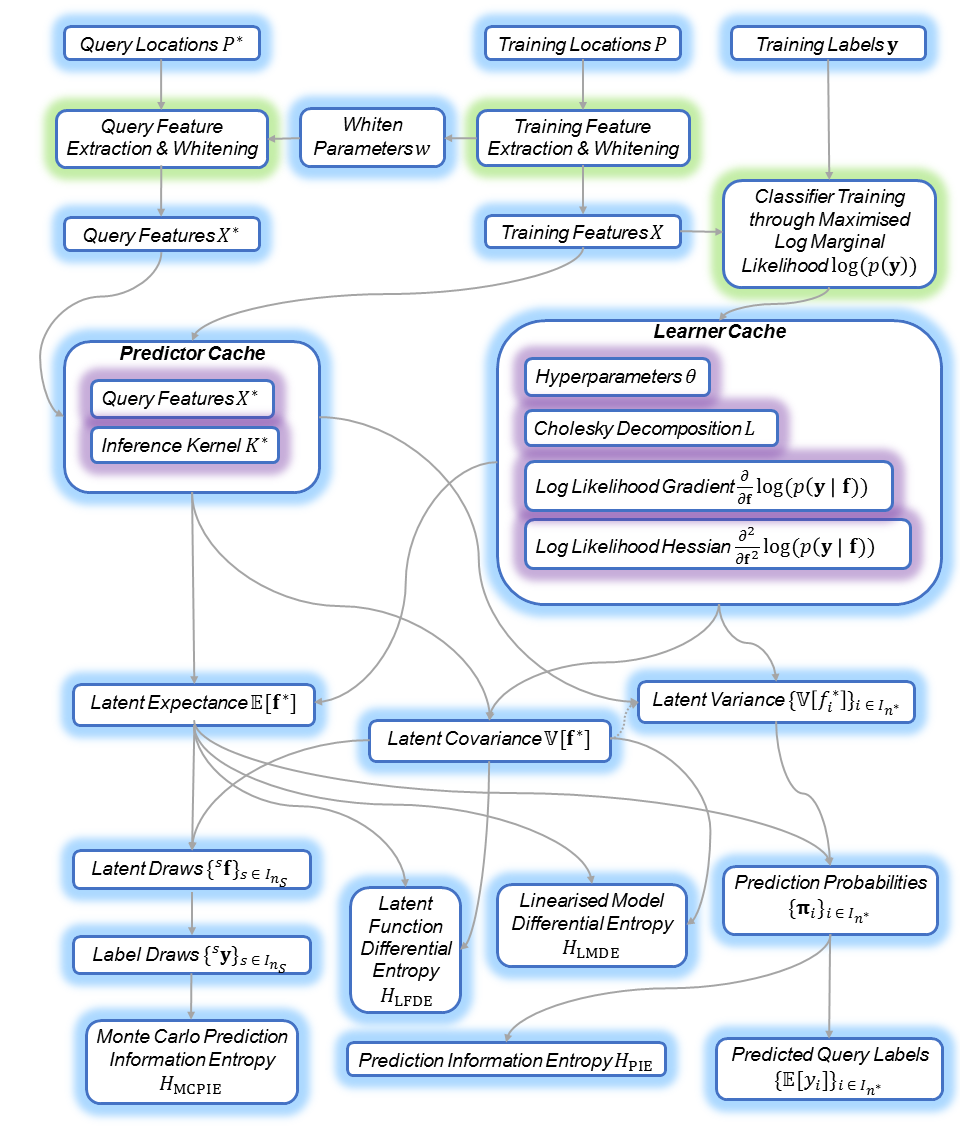
\includegraphics[width = 0.8\linewidth]{Figures/inferenceflow.eps}
		\caption{Inference Information Flow}
		\label{Figure:InferenceFlow}
		\end{figure}	

		As the figure suggests, the mapping process is a supervised learning problem for which the habitat labels $\bvec{y}^{\star}$ at the query locations $P^{\star}$ is to be inferred from the query features $X^{\star}$ by learning a relationship between the habitat labels $\bvec{y}$ and the training features $X$ at the training locations $P$. Only the {\color{Gray} gray} and {\color{ForestGreen} green} coloured arrows in Figure \ref{Figure:InferenceFlow} are necessary for mapping to be achieved.
		
		As the discussion continues in the following two chapters, each part of the diagram will be expanded and addressed.
		
	\section{Bathymetric Features}
	\label{BenthicHabitatMapping:BathymetricFeatures}
	
		This thesis can be broken down into two main parts - benthic habitat mapping and informative path planning. Benthic habitat mapping itself includes bathymetric feature extraction, and habitat class inference. Thus, benthic habitat mapping refers to the two stage process of feature extraction and habitat class inference, with the latter being the main bottleneck for this process. This section will focus on bathymetric feature extraction and modeling.
			
		In order for autonomous underwater vehicles to infer a map of the benthic habitats, and later plan a path to increase mapping accuracy, it would need a method to predict the types of environments it may encounter, with a measure of its prediction uncertainty.
		
		While the path planner is to plan in the spatial space, in general the prediction model operates upon some feature space with more direct and explicit relationships with the output to be inferenced.
		
		It is thus important to make a distinction between the feature space $\mathcal{X}$ for which benthic habitat modeling is to occur and the spatial space $\mathcal{P}$ for which bathymetric modeling and planning is to occur. The spatial space usually consists of Cartesian coordinates $(x, y)$ in the eastings-northings frame or the longitude-latitude frame, so that $\mathcal{P} \subseteq \mathbb{R}^{2}$. The path is to be planned in this spatial space. The frame is usually converted into a local body frame during the execution of control signals for path tracking. However, this does not affect the formulation presented here. The feature space $\mathcal{X} \subseteq \mathbb{R}^{p}$, where $p$ is the number of features (feature dimensions), includes bathymetric features for which the habitat labels will be modeled upon. Depending on the features employed for the modeling process, there are usually approximate analytical forms for extracting such features from raw depth observations.
		
		The following bathymetric features shown in \cref{Table:BathymetricFeatures} were selected for habitat mapping. The benthic habitats would be modelled upon five bathymetric features - bathymetric depth, aspect (short scale), rugosity (short scale), aspect (long scale), and rugosity (long scale). Spatial coordinates are chosen to be excluded from the bathymetric feature set. For benthic habitat mapping, it is expected that ecological habitats and geological sites exhibit no explicit relationship with the location of the site, and that its properties arise solely due to the local terrain structure and seafloor characteristics  of that site. This means that the nature of the habitat depends on the location implicitly through explicit dependence on bathymetric structure of the seafloor. These five bathymetric features summarises the local terrain structure at every location of the seafloor, and forms our feature space $\mathcal{X} \subseteq \mathbb{R}^{5}$ with $p = 5$.
		
		\begin{table}[h]
			\begin{center}
				\begin{tabular}{ l c c }
					\hline
					\hline
					Feature Name & Feature Symbol & Feature Units \\
					\hline
					\hline
					Depth & $z$ & m \\
					Aspect (Small Scale) & $a_{s}$ & m/m \\
					Aspect (Large Scale) & $a_{l}$& m/m \\
					Rugosity (Small Scale) & $r_{s}$ & $\mathrm{m^{2}/m^{2}}$ \\
					Rugosity (Large Scale) & $r_{l}$ & $\mathrm{m^{2}/m^{2}}$  \\
					\hline
					\hline
				\end{tabular}
			\end{center}
	  	\caption{Bathymetric Features}
	  	\label{Table:BathymetricFeatures}			
	  	\end{table}	
		
		Aspect also refers to the slope of the seafloor terrain, while rugosity is a measure of small-scale variations or amplitude in the height of a surface.
		
		The raw bathymetric data contains depth information at various spatial locations. Such data are often collected rather uniformly in approximate grid formations such that it is possible to calculate the ocean floor slope through finite differencing. The aspect, or slope, is divided into small scale and large scale variations, as marine environments - especially underwater habitats - often depend not only on the immediate slope but also slope variations on the larger scale. The same idea applies to rugosity to measure local height variations at two different scales.
		
		% Define block styles
		\tikzstyle{block} = [rectangle, draw, fill = green!10!blue!20, text width = 7.5em, text centered, rounded corners, minimum height = 4em]
		\tikzstyle{line} = [draw, -latex']
	
		\begin{figure}[!ht]
		\centering\makebox[\textwidth]{
			\begin{tikzpicture}[node distance =4cm, auto,
			comment/.style={
			rectangle, 
			inner sep= 5pt, 
			text width=4cm, }]
			
			\node [block] (spatialspace) {Seafloor Spatial Space $\mathcal{P}$};
			\node [block, right of = spatialspace] (featurespace) {Bathymetric Feature Space $\mathcal{X}$};
			\node [block, right of = featurespace] (mapspace) {Habitat Map Space $\mathcal{Y}$};
					
			\draw [line] (spatialspace) -- (featurespace);
			\draw [line] (featurespace) -- (mapspace);
			
			\draw [decorate ,decoration = {brace, amplitude = 10pt, raise = 3mm}]
			(spatialspace.85) -- (featurespace.95) node [black, midway, yshift = 10mm]
			{Bathymetric Feature Extraction};
			
			\draw [decorate, decoration = {brace, amplitude = 10pt, raise = 3mm}, xshift = 0pt, yshift = 0pt]
			(featurespace.85) -- (mapspace.95) node [black, midway, yshift = 6mm] 
			{Habitat Class Inference};
						
			\end{tikzpicture}}		
		\caption{Benthic Habitat Mapping Process}
		\label{Figure:BenthicHabitatMappingProcess}
		\end{figure}
		
		Figure \ref{Figure:BenthicHabitatMappingProcess} show a high level overview of the benthic habitat mapping process. As bathymetric data is available in more quantities and distributed more uniformly, it is often sufficient to employ the feature extraction process outlined in \cref{BenthicHabitatMapping:BathymetricFeatures:FeatureExtraction} to obtain the bathymetric features for modeling. However, if the bathymetric data is sufficiently sparse or is not distributed uniformly for grid based methods, then the feature extraction process itself becomes a prediction problem.

		In that case, a Gaussian process regression model is proposed for predicting the features at a given spatial location. While this is much more computationally expensive than performing feature extraction, it is also quite rare that this is necessary under abundant bathymetric data. In most cases, it suffices to simply take the nearest neighbouring feature.		
		
		\subsection{Formulation}
		
			With the basic structure of the benthic habitat mapping process presented above, the model spaces involved can now be formulated formally.
			
			As established previously, the spatial space $\mathcal{P} \subseteq \mathbb{R}^{2}$ and feature space $\mathcal{X} \subseteq \mathbb{R}^{5}$ are compact subsets of $\mathbb{R}^{2}$ and $\mathbb{R}^{5}$ respectively. On the other hand, the habitat map space $\mathcal{Y} \subset \mathbb{N}$ is a strict finite subset of the the natural numbers, with each distinct integer representing a particular habitat type.
			
			Further, define $\mathscr{P} := \mathscr{P}(\mathcal{P})$, $\mathscr{X} := \mathscr{X}(\mathcal{X})$, and $\mathscr{Y} := \mathscr{Y}(\mathcal{Y})$ as the $\sigma$-algebras generated by $\mathcal{P} \subseteq \mathbb{R}^{2}$, $\mathcal{X} \subseteq \mathbb{R}^{5}$, and $\mathcal{Y} \subset \mathbb{N}$ respectively. Specifically, this means that $X \in \mathscr{X}$ implies $X \subseteq \mathcal{X}$, and similarly for $\mathscr{P}$ and $\mathscr{Y}$.
			
			Note that if $X := \{\bvec{x}_{i}\}_{i \in I_{n}} := \{\bvec{x}_{1}, \bvec{x}_{2}, \dots, \bvec{x}_{n}\} \in \mathscr{X}$ is a \textit{finite} collection of feature vectors $\bvec{x}_{i} \in \mathcal{X}$ for all $i \in I_{n}$, then $X$ is equivalent to the matrix $[\bvec{x}_{1}, \bvec{x}_{2}, \dots, \bvec{x}_{n}]^{T} \in \mathbb{R}^{n \times p}$. For notational and analytical convenience, the two quantities will be considered equivalent such that $X := \{\bvec{x}_{i}\}_{i \in I_{n}} := \{\bvec{x}_{1}, \bvec{x}_{2}, \dots, \bvec{x}_{n}\} \equiv [\bvec{x}_{1}, \bvec{x}_{2}, \dots, \bvec{x}_{n}]^{T}$. This notation is used consistently throughout, and a similar formulation applies to spatial coordinates $P \in \mathscr{P}$. For target labels in the habitat map space, $\bvec{y} := \{y_{i}\}_{i \in I_{n}} := \{y_{1}, y_{2}, \dots, y_{n}\} \in \mathscr{Y}$ is already consistent with existing nomenclature for vectors, and also complies in form with the above matrix formulation. Recall that for an arbitrary quantity $q_{i}$ indexed by $i \in I_{n}$, $\{q_{i}\}_{i \in I_{n}}$ is defined to be $\{q_{1}, q_{2}, \dots, q_{n}\}$ which is equivalent to a vector if $q_{i}$ is a scalar and a matrix if $q_{i}$ is a vector.
		
		\subsection{Data Matching}
		\label{BenthicHabitatMapping:BathymetricFeatures:DataMatching}
		
			A subtlety that arises from the above formulation is that during the training stage, the bathymetric data and the label data are not necessarily observed at the same places. Figure \ref{Figure:ScottReefBathymetricFeatures} illustrates the spatial distribution of the two datasets in a typical setting using the Scott Reef data set \citep{IMOS} as an example.
		
			\begin{figure}[!htbp]
			\centering
				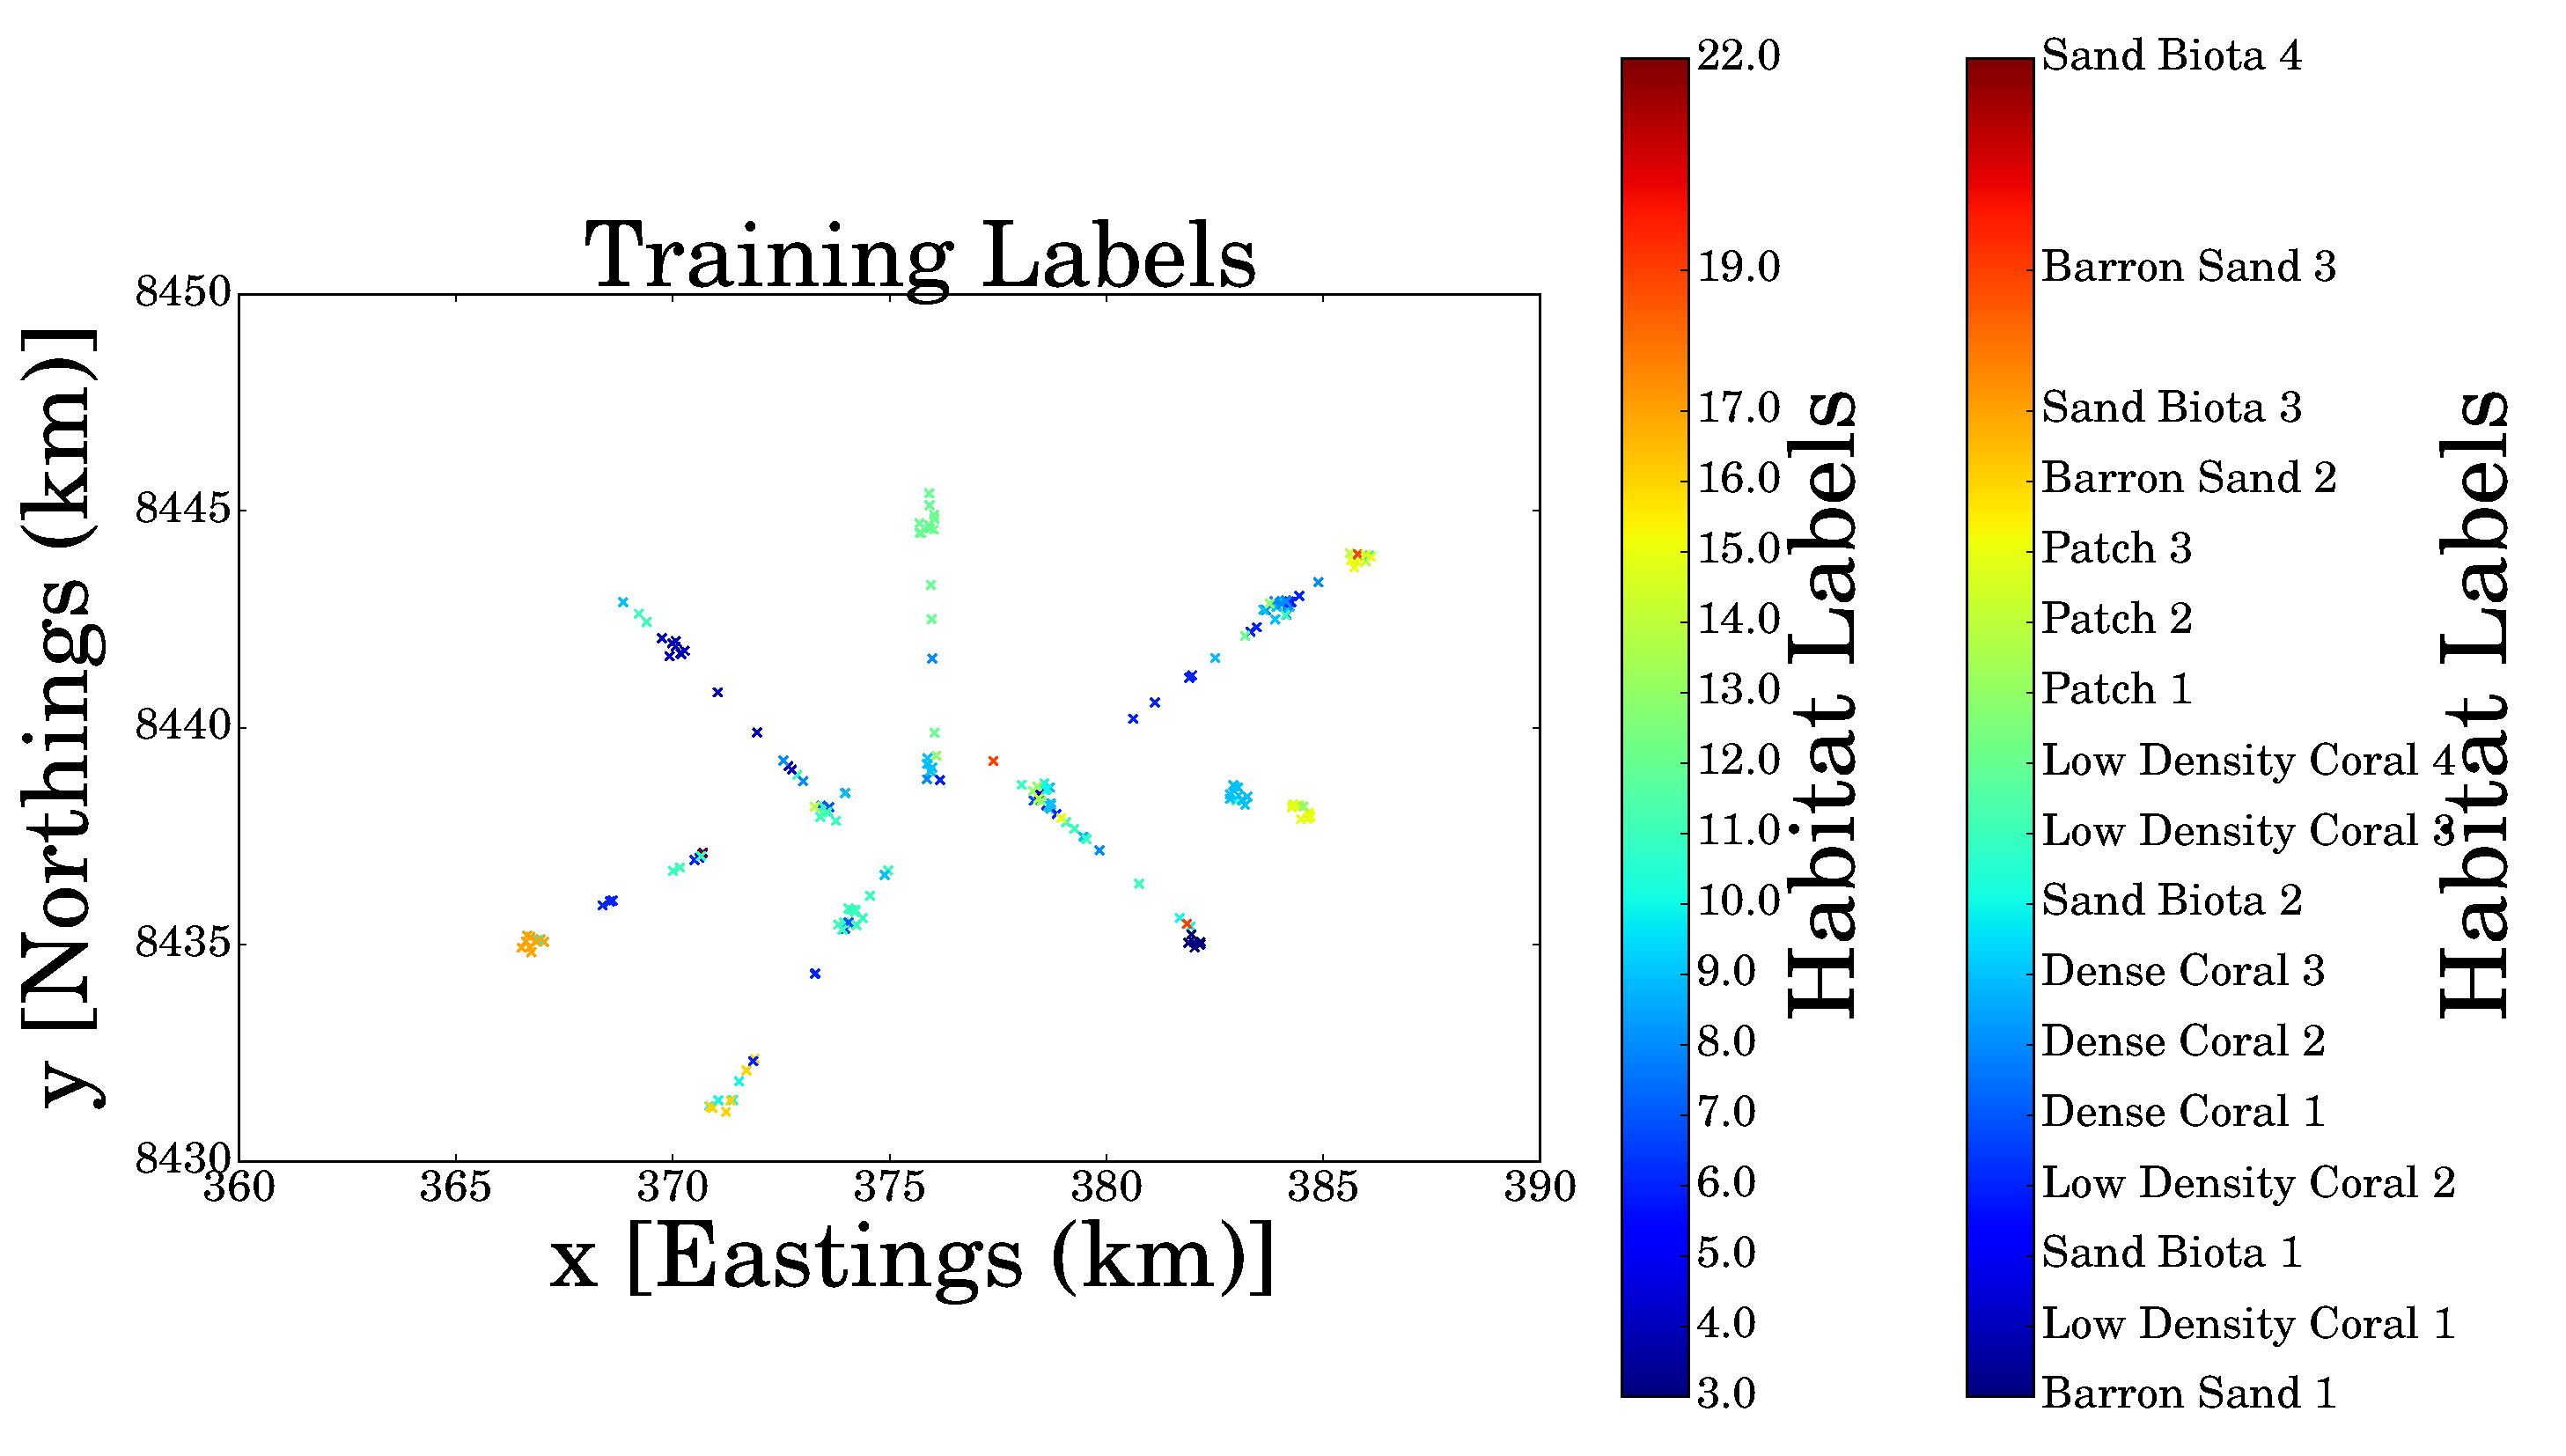
\includegraphics[width = 0.32\linewidth]{Figures/scott_reef_modeling/Figure1.eps}
				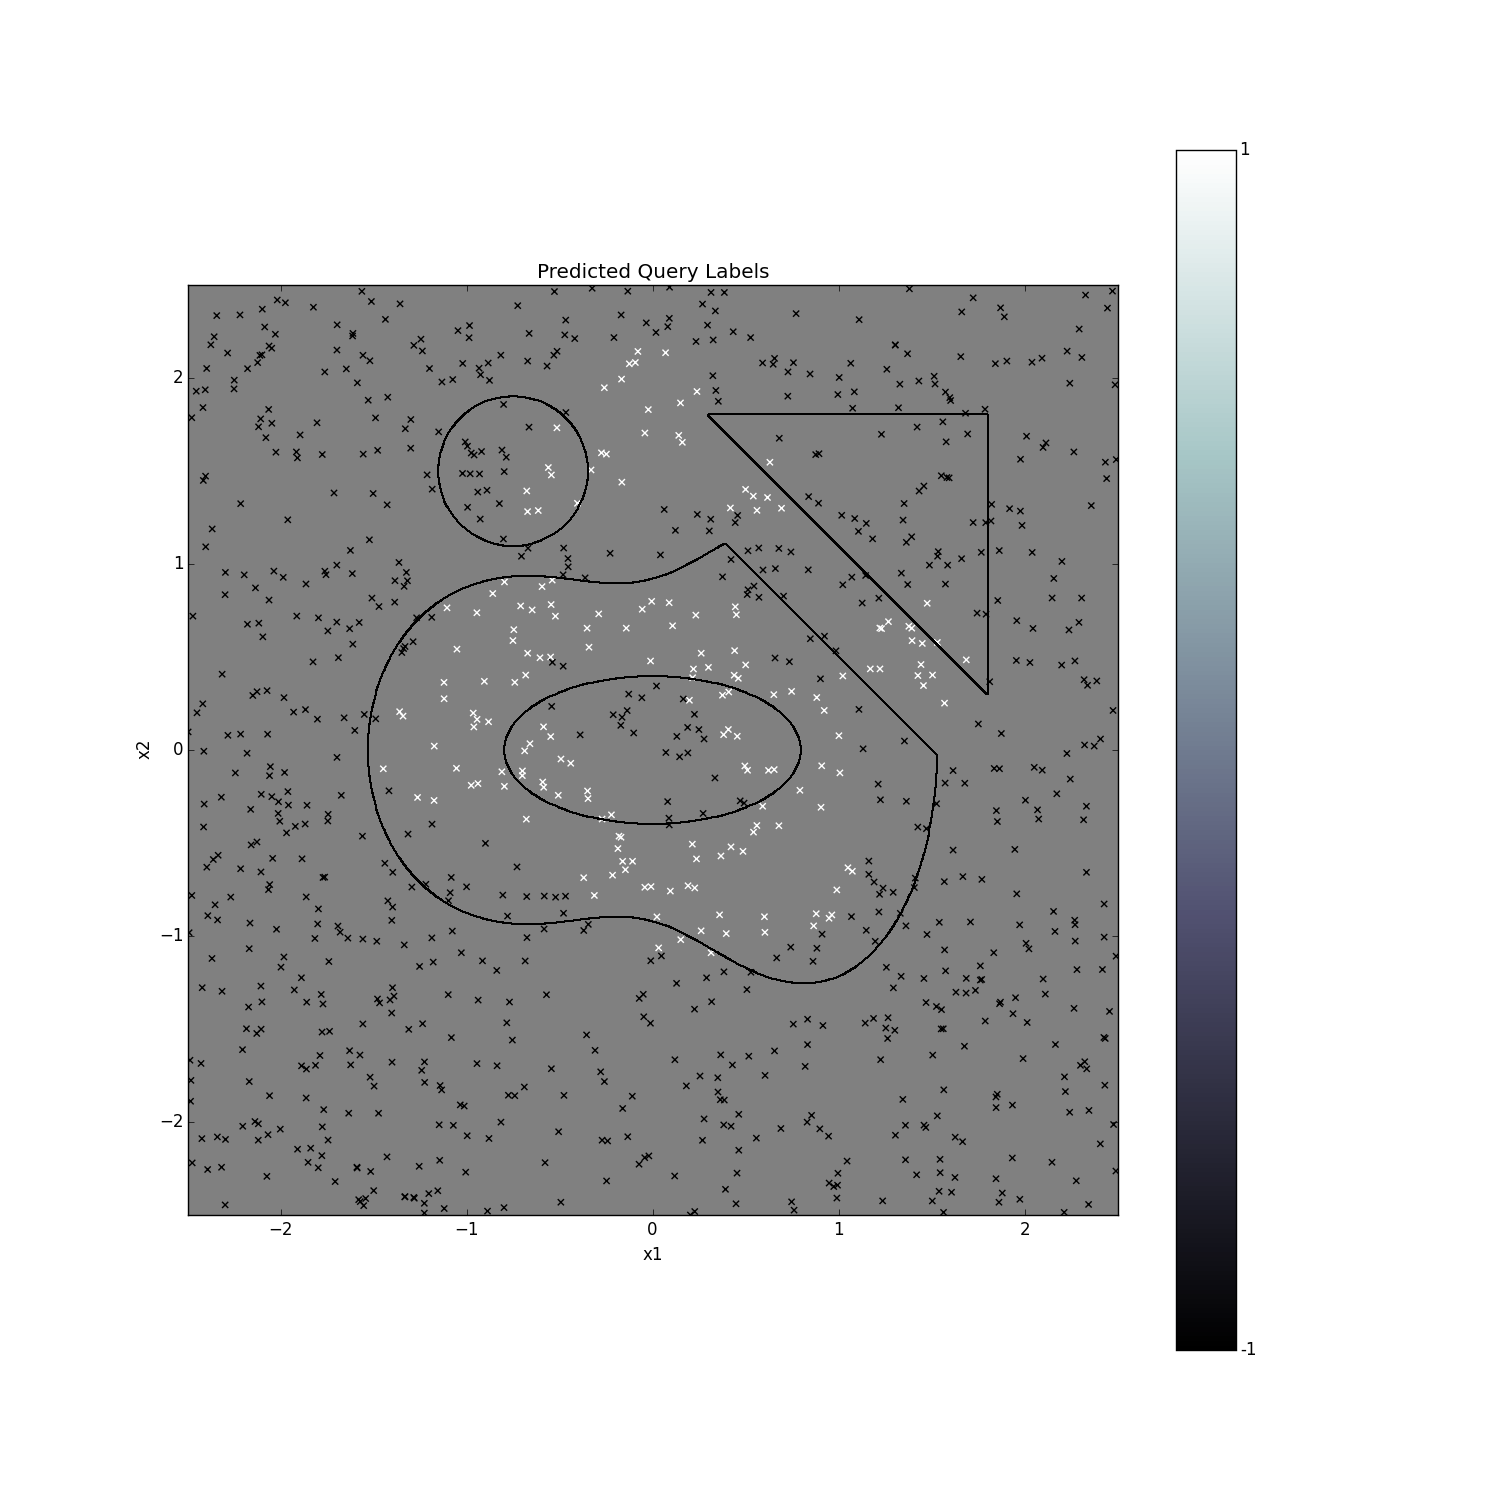
\includegraphics[width = 0.32\linewidth]{Figures/scott_reef_modeling/Figure2.eps}
				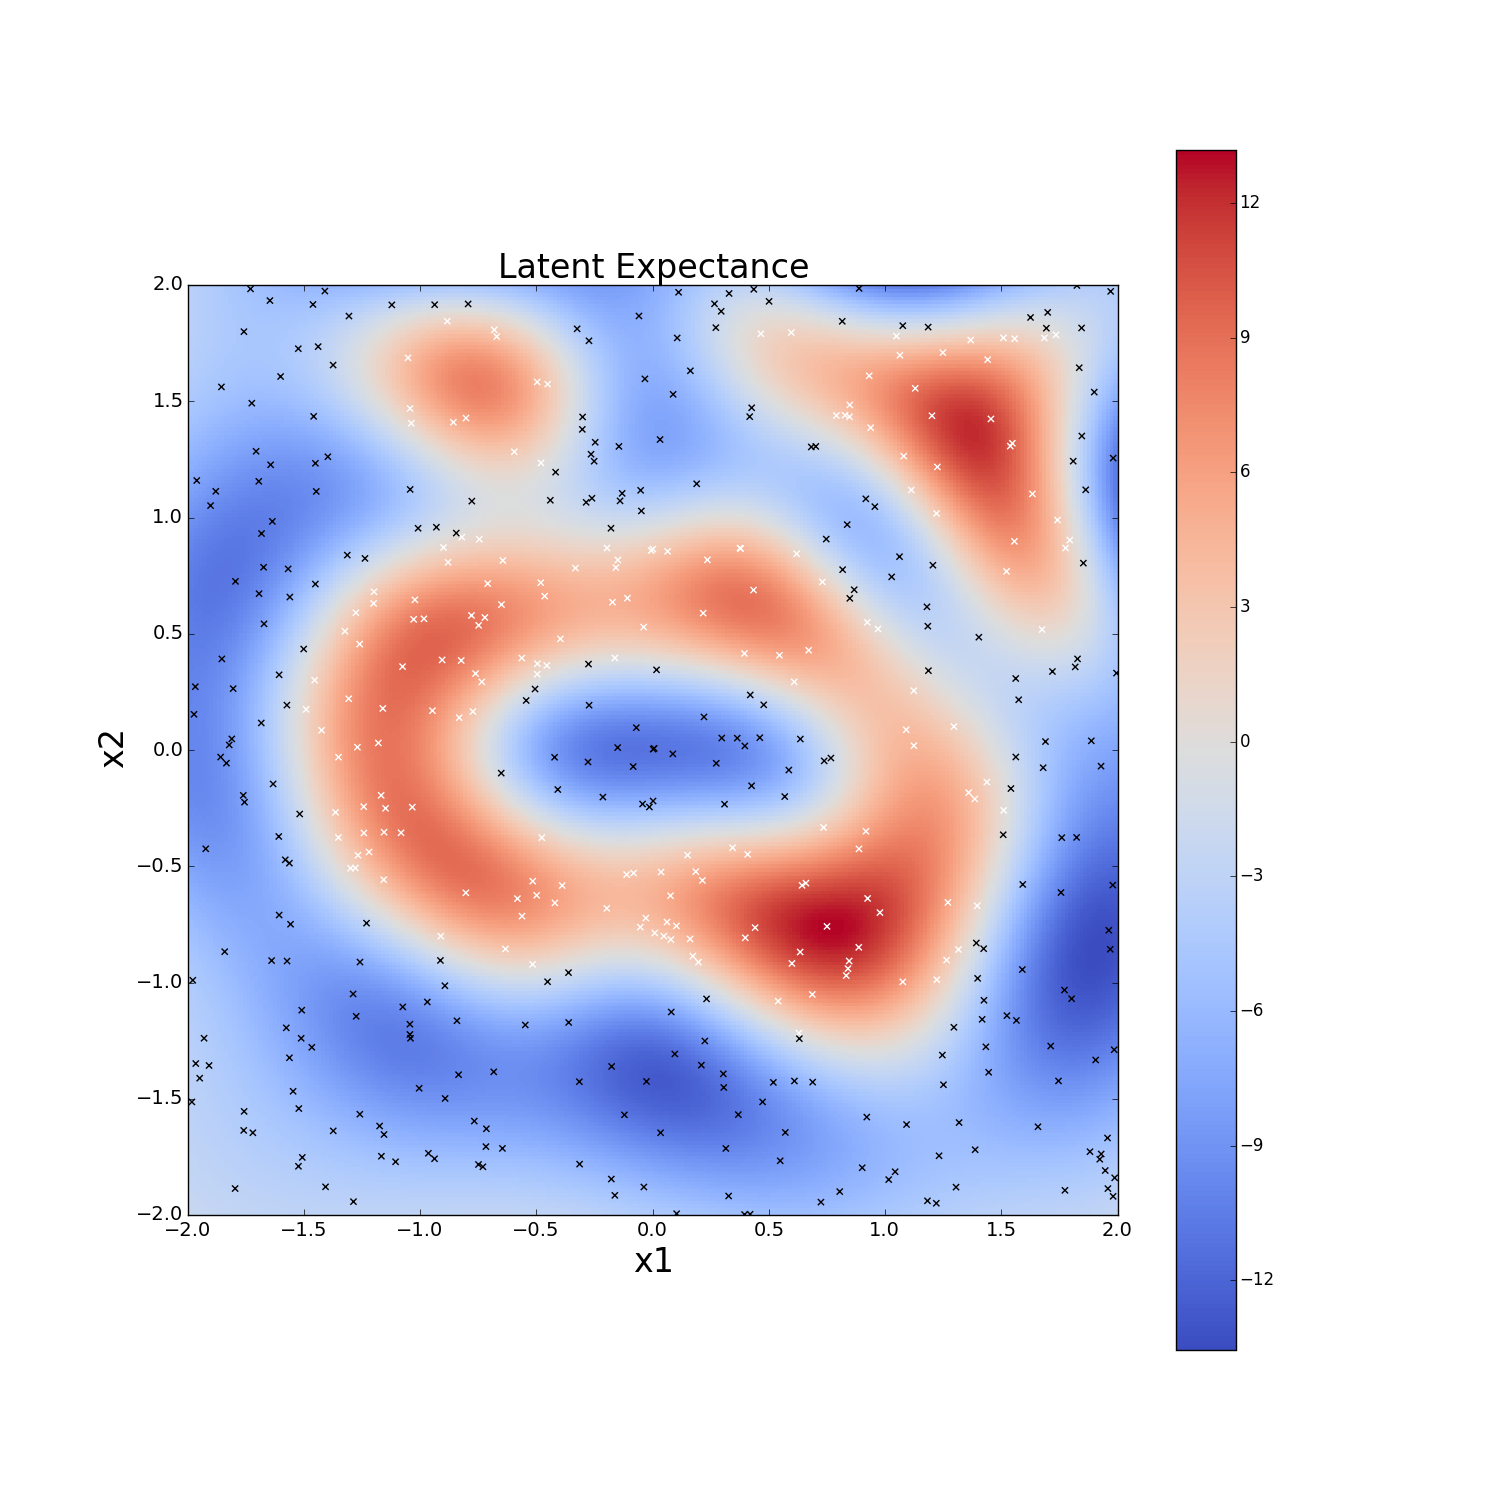
\includegraphics[width = 0.32\linewidth]{Figures/scott_reef_modeling/Figure3.eps}
				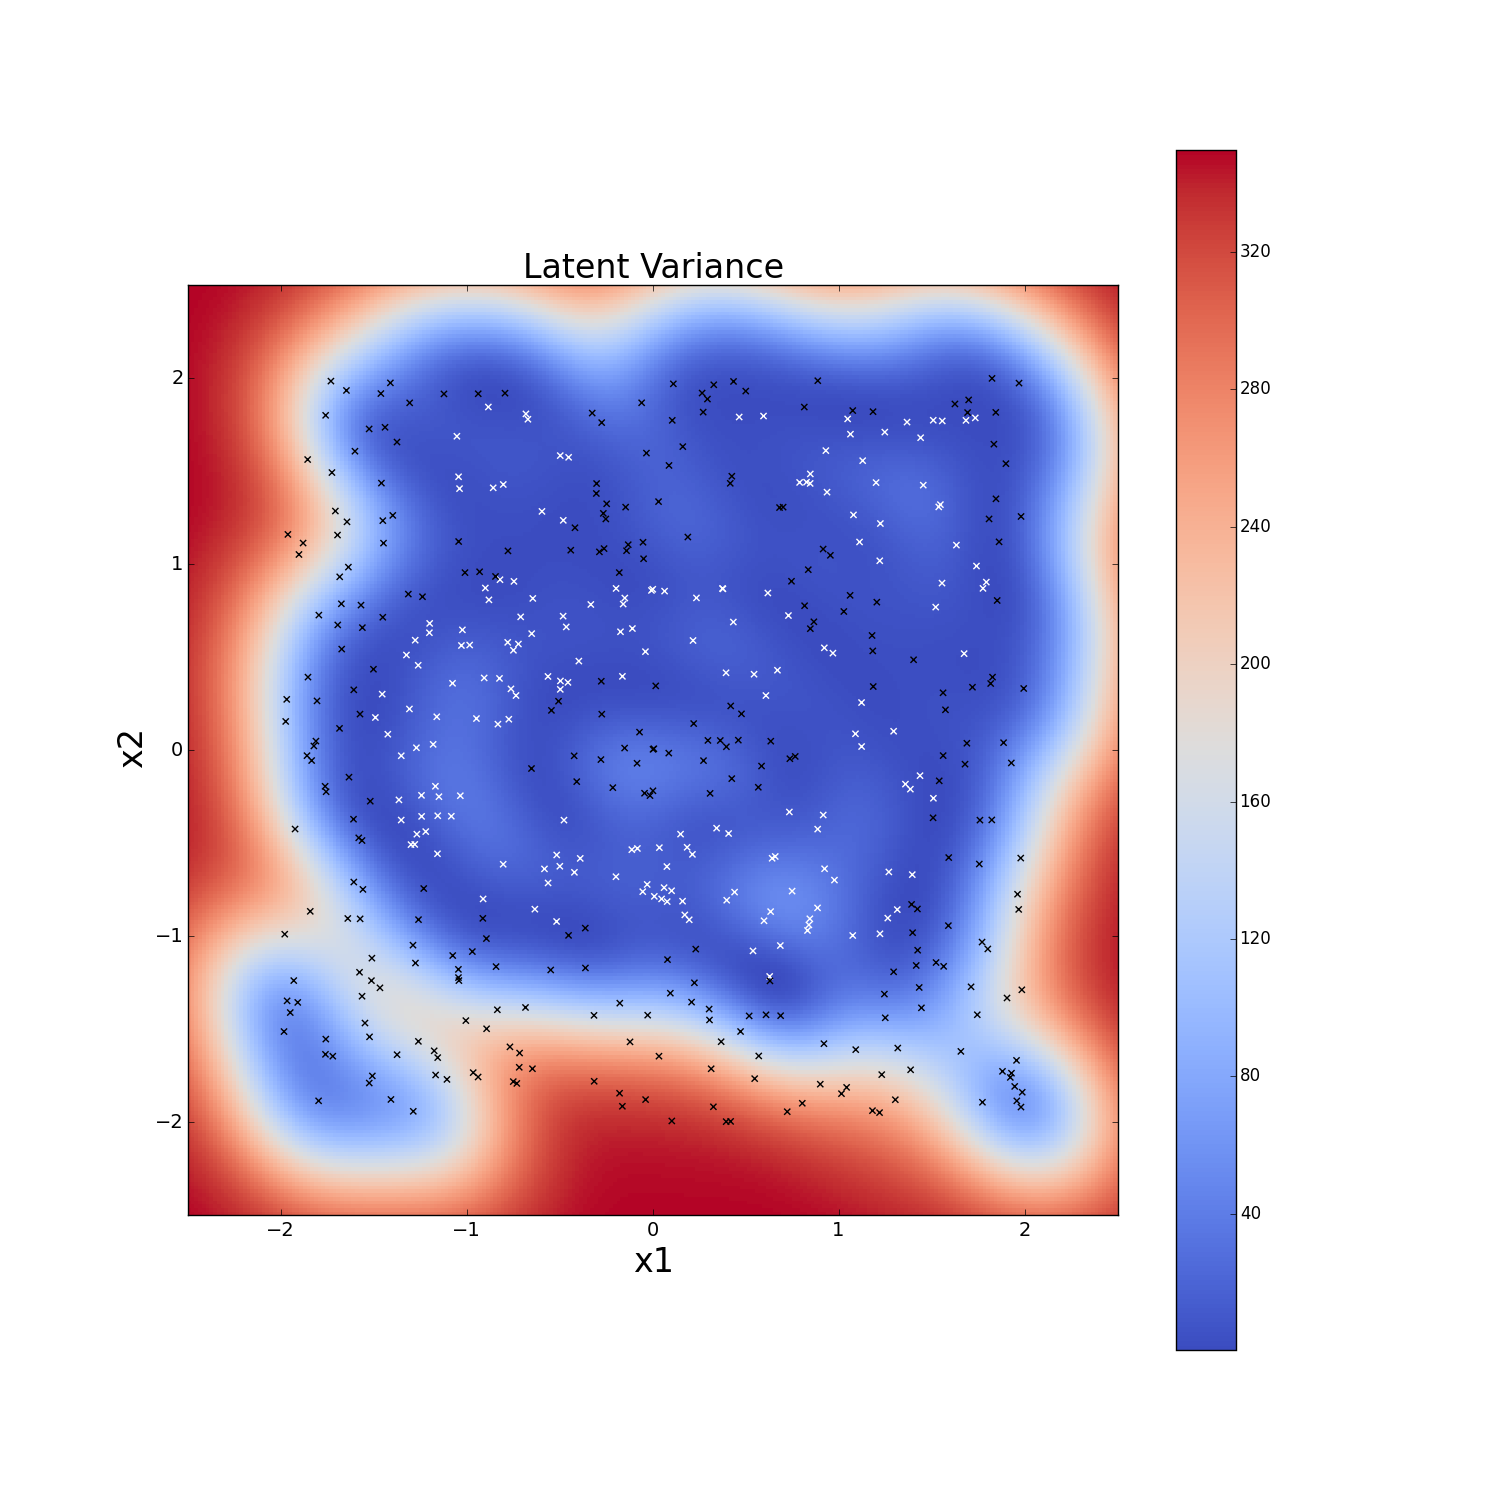
\includegraphics[width = 0.32\linewidth]{Figures/scott_reef_modeling/Figure4.eps}
				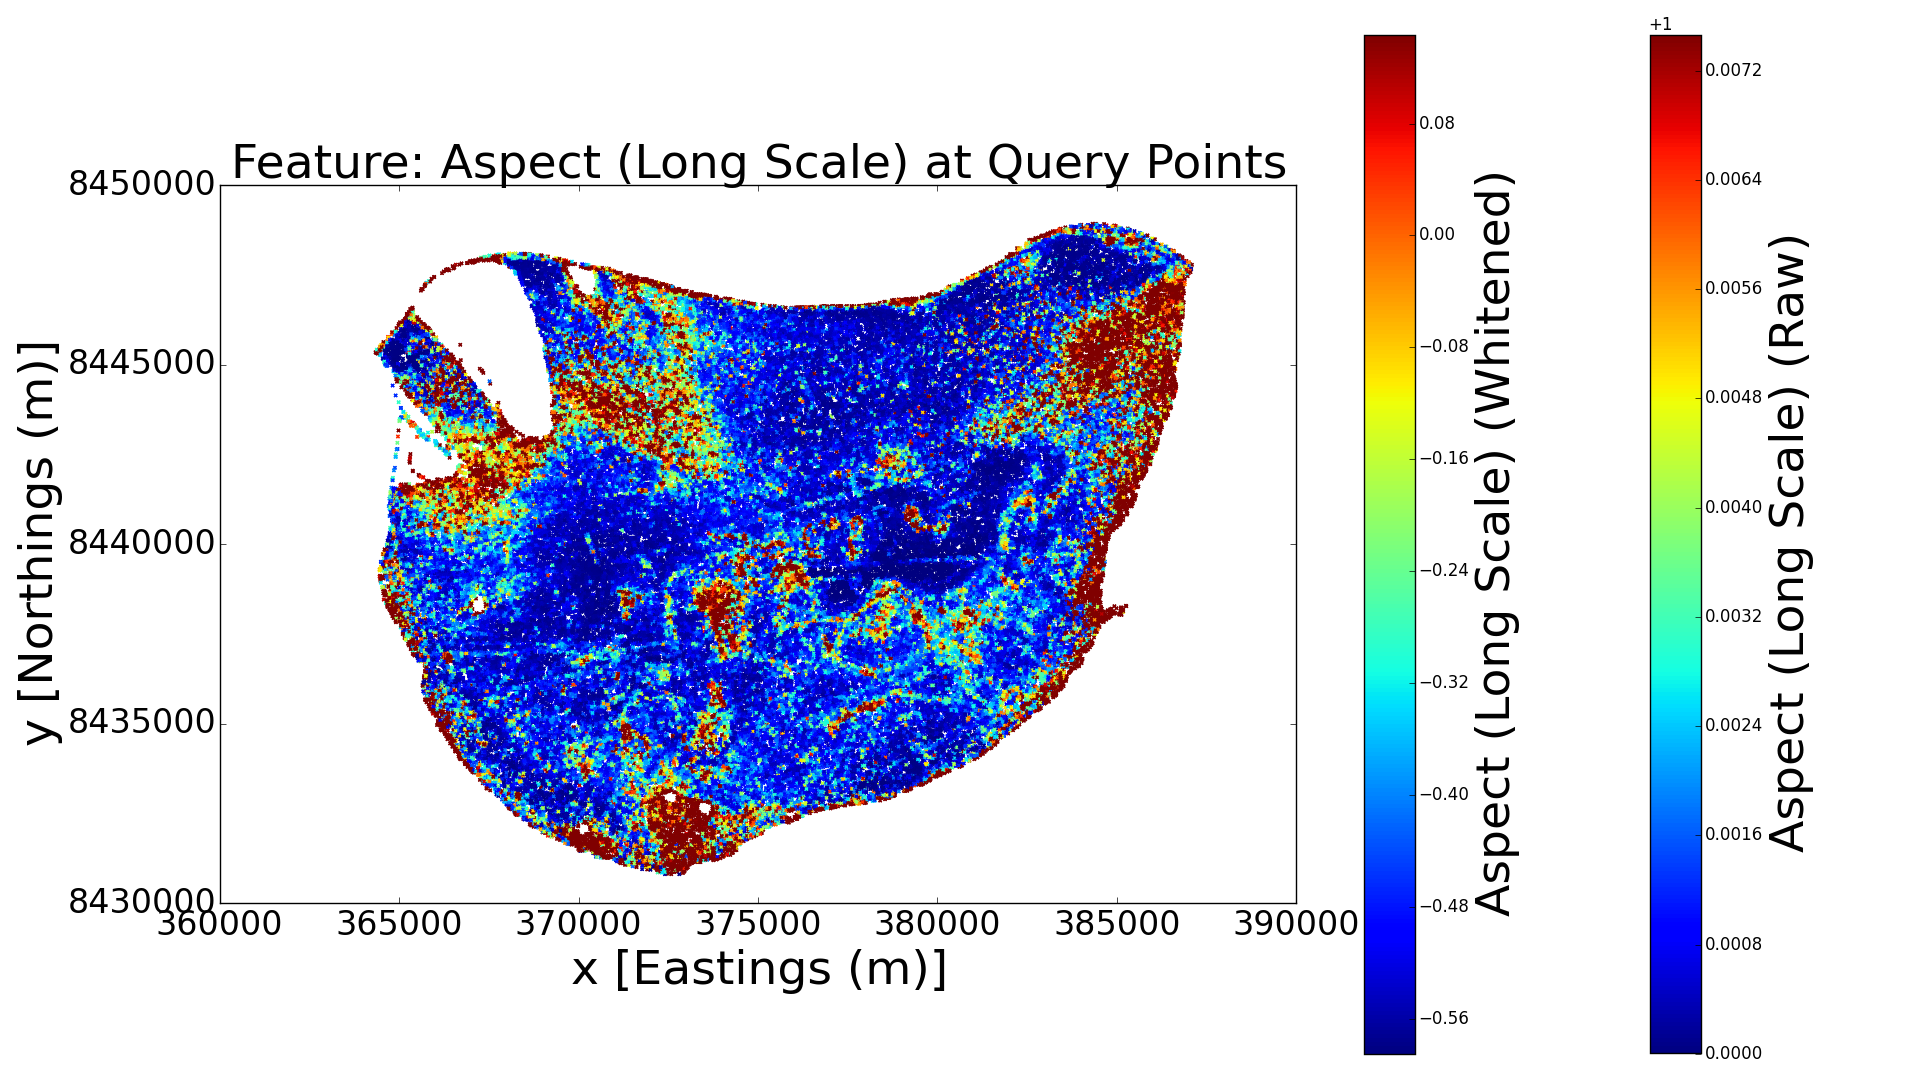
\includegraphics[width = 0.32\linewidth]{Figures/scott_reef_modeling/Figure5.eps}
				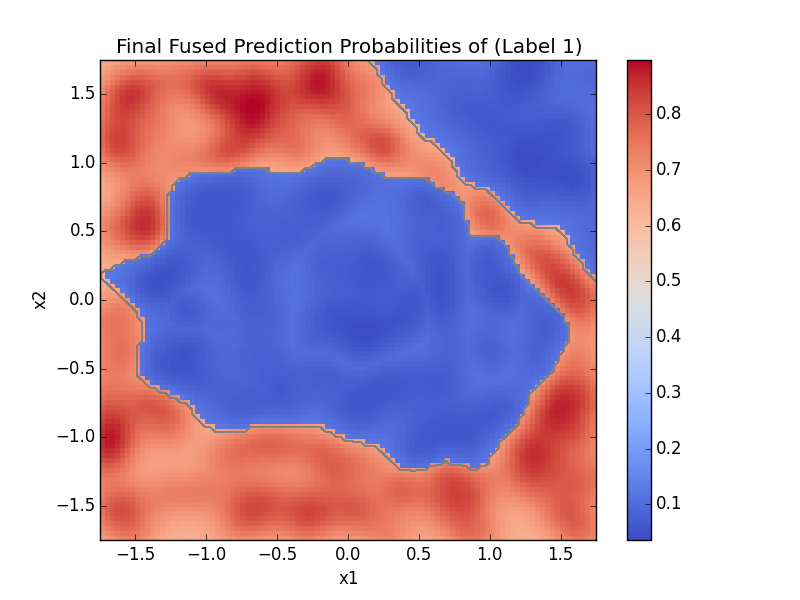
\includegraphics[width = 0.32\linewidth]{Figures/scott_reef_modeling/Figure6.eps}
			\caption{Scott Reef Bathymetric Features}
			\label{Figure:ScottReefBathymetricFeatures}
			\end{figure}
			
			In the Scott Reef case, the bathymetric observations span the entire region of interest densely. However, while bathymetric data are usually collected rather uniformly and densely, the label data are collected from past AUV missions whose trajectory are continuous paths across the ocean floor \citep{Squidle}. Often times, these paths are approximate line segments which cover a very limited portion of the region of interest. Due to slower AUV velocity as compared to surface ships which often employ SONAR or LIDAR techniques for bathymetry mapping, the label data are also spatially denser and concentrated on the mission trajectory, while being almost non-existent elsewhere, making it a multi-modal distributed dataset. 
			
			Therefore, in order for the GP classifier to learn the relationship between the bathymetric features and habitat labels, the bathymetric data and label data must have a one-to-one correspondence. In other words, they must exist at the same locations. 
			
			Formally, let $P_{b}, P_{h} \in \mathcal{P}$ be the spatial positions at which bathymetric data and habitat label data have been observed. Let $X_{b} \in \mathcal{X}$ be the bathymetric features observed at $P_{b}$ and $\bvec{y}_{h} \in \mathcal{Y}$ be the habitat labels observed at $P_{h}$. The data matching problem is to obtain or infer $X_{h} \in \mathcal{X}$, the bathymetric features at locations $P_{h}$, from $X_{b}$.
			
			This is a standard supervised learning problem. Specifically, the aim is to learn an inference model $\zeta: P_{h} \mapsto X_{h}$ from the empirical relationship $P_{b} \mapsto X_{b}$.
			
			While it is possible to employ a separate GP regressor to perform the above inference, this adds unnecessary computational complexity. Since GPs are $O(n^{3})$ algorithms, using a layered GP approach where both stages of the benthic habitat mapping process employs GPs will increase the inference bottleneck.
			
			Instead, as there exists an abundance of bathymetric data, without much loss of accuracy it suffices to employ a nearest neighbour interpolation to obtain $X_{h}$. 
			
%			Therefore, in order to predict label data, the training data would need to be matched accurately. There are two straight forward choices at hand. The first is to estimate the bathymetric features at places where label data exists. However, at places near past mission paths, bathymetric data appears much more sparsely than label data, so that the feature extraction or regression prediction will yield very similar features across manly label data points. This reduces prediction power through a slow varying and limited feature group.
%			
%			Instead, the second choice is to estimate the label data at places where bathymetric data exists. In this setting, regions closer to past mission paths have higher volumes of label data, increasing the amount of training points. Regions further away would naturally generate more prediction uncertainty in the prediction stage.
%			
%			Hence, second method is chosen to be employed for data matching, in order to form our training set. Naturally, to predict environment labels from bathymetric features, we again need the Gaussian process classification model.
			
			\FloatBarrier
	
		\subsection{Feature Extraction}
		\label{BenthicHabitatMapping:BathymetricFeatures:FeatureExtraction}
		
			The feature extraction process assumes that the bathymetric depth data is available in grid form. That is, one can represent the available depth data $Z = \{z_{k}\}_{k \in {1, 2, ..., N}}$ as $Z = \{z_{ij}\}_{i \in {1, 2, ..., n_{i}}, \;\; j \in {1, 2, ..., n_{j}}}$ where varying $i$ and $j$ corresponds to varying data points in axis 1 and 2 respectively. Axis 1 and 2 is required to form an orthonormal frame. While axis 1 and 2 is usually aligned with the eastings-northings frame, it is generally not required for the feature extraction process.
			
			Without loss of generality, let $x$ and $y$ denote quantities corresponding to the orthogonal axes. We have that at $(x_{i}, y_{j})$ $(i \in {1, 2, ..., n_{i}}, \;\; j \in {1, 2, ..., n_{j}})$ the depth is measured as $z_{ij}$. The partial derivatives of various degrees of accuracy and scale can then be estimated through central differencing, as shown in \cref{Table:AspectExtraction}. The table shows the case for extracting aspect in the $x$-direction. Correspondingly, replacing the operations from $i$ to $j$ the aspect in the $y$-direction can also be similarly extracted.
			
			\bgroup
			\def\arraystretch{2}%  1 is the default, change whatever you need
			\begin{table}[h]
				\begin{center}
					\begin{tabular}{ c c }
						\hline
						\hline
						N & Aspect (Slope) Extraction [$x$-direction]\\
						\hline
						\hline
						3 & $^{3}_{x}a_{i, j} := \frac{- z_{i - 1, j} + z_{i + 1, j}}{2h}$ \\
						5 & $^{5}_{x}a_{i, j} := \frac{z_{i - 2, j} - 8 z_{i - 1, j} + 8 z_{i + 1, j} - z_{i + 2, j}}{12h}$ \\
						7 & $^{7}_{x}a_{i, j} := \frac{-z_{i - 3, j} + 9 z_{i - 2, j} - 45 z_{i - 1, j} + 45 z_{i + 1, j} - 9 z_{i + 2, j} + z_{i + 3, j}}{60h}$ \\
						9 & $^{9}_{x}a_{i, j} := \frac{3 z_{i - 4 j} - 32 z_{i - 3, j} + 168 z_{i - 2, j} - 672 z_{i - 1, j} + 672 z_{i + 1, j} - 168 z_{i + 2, j} + 32 z_{i + 3, j} - 3 z_{i + 4, j}}{840h}$ \\
						\hline
						\hline
					\end{tabular}
				\end{center}
		  	\caption{Aspect feature extraction using finite (central) difference approximations}
		  	\label{Table:AspectExtraction}			
		  	\end{table}	
	  		\egroup
	  		
	  		The chosen spacing employed in this thesis are $N = 3$ neighbors for short scale aspect and $N = 9$ neighbors for large scale aspect. That is, \begin{align*} \numberthis \label{Equation:AspectExtraction}
	  				{_{x}\{a_{s}\}_{i, j}} &:= {^{3}_{x}a_{i, j}} \quad && {_{y}\{a_{s}\}_{i, j}} := {^{3}_{y}a_{i, j}} \quad && {\{a_{s}\}_{i, j}} := \sqrt{{_{x}\{a_{s}\}^{2}_{i, j}} + {_{y}\{a_{s}\}^{2}_{i, j}}} \\
	  				{_{x}\{a_{l}\}_{i, j}} &:= {^{9}_{x}a_{i, j}} \quad && {_{y}\{a_{l}\}_{i, j}} := {^{9}_{y}a_{i, j}} \quad && {\{a_{l}\}_{i, j}} := \sqrt{{_{x}\{a_{l}\}^{2}_{i, j}} + {_{y}\{a_{l}\}^{2}_{i, j}}}
	  		\end{align*}
	  						  					
			Central differencing is chosen as it is more numerically accurate. The disadvantages of instability and slightly higher time complexity from dynamic cases are not present in the static feature extraction process. Nevertheless, forward differencing is to be used at the boundaries of the dataset where neighboring data is missing on one side.
						
			With two axis, the result is a 2 element gradient vector. It is possible to treat the 2 elements as separate features. However, this would make the modeling problem frame dependent which would unnecessarily complicate the modeling process. Therefore, the magnitude of this gradient is taken as the aspect feature \eqref{Equation:AspectExtraction}. 
			
			Rugosity is a measure of local height variations in the terrain. By definition, it is computed with $r = A_{r}/A_{g}$, the real surface area divided by the geometric surface area. Under bathymetry measurements that are geo-referenced through stereo imagery, rugosity can be calculated through a Delaunay triangulated surface mesh and projecting areas onto the plane of best fit using Principal Component Analysis (PCA) \citep{Friedman:Rugosity}.
							
			\FloatBarrier
				
	\section{Approximation methods for GP Classification}
	
		\subsection{Laplace Approximation}
		
		\subsection{Probabilistic Least Squares Approximation}
		
		\subsection{Properties \& Performance}
		
			% Laplace Approximation and Probabilistic Least Squares
			Compare probability outputs, classification outputs, entropy outputs, etc
		
	\section{Methods for Multiclass Classification}
	
		\subsection{One Versus All Classification}
		
			While a consistent framework for the GP Multi-class classification using Laplace approximation exist, a simpler and perhaps a more computationally efficient approach is to employ the One v.s. All (OVA) and All v.s. All (AVA) philosophy. The following discussion assumes that there are $c > 2$ classes of labels for which classification is to occur. 
				
			The OVA approach performs classification by introducing $c$ \textit{independent} classification problems, each trying to classify a label against all others. Each of these problems are thus a binary classification problem for which solution methods are known. Once the predictive probabilities from all learned GP classifiers are obtained, a consistent framework is used for fusing the separate prediction probabilities into a coherent prediction probability. This is necessary as the binary classifiers are independently learned and performs prediction independently, and may not necessarily provide coherent results. In fact, simply stacking the prediction probabilities together yields a "probability" distribution that does not sum up to 1.
				
			The AVA approach operates similarly. It insteads introduces $\frac{c (c - 1)}{2}$ \textit{independent} classification problems, each classifying between a pair of labels. The same exact philosophy follows in that a final consistent framework is needed for fusing the prediction probabilities into one coherent prediction probability. It is often more difficult for probability fusion in the AVA setting as compared to the OVA setting
				
		\subsection{All Versus All Classification}
			
		\subsection{Properties \& Performance}
	
	\section{Probability Fusion Methods}
	
		\subsection{Simple Normalisation}
			
		\subsection{Mode Keeping}
			
		\subsection{Exclusion}
			
	\section{Mapping Scott Reef Benthic Habitats}
	\label{BenthicHabitatMapping:ScottReef}
	
		
		The Scott Reef data set is provided by \cite{IMOS}. The benthic labels are clustered in an unsupervised manner from benthic imagery using Gaussian latent Dirichlet allocation (LDA) \cite{Steinberg2015128}, producing 22 unique benthic class labels, with 17 of them associated with identifiable semantic meaning and the rest either over-exposed or under-exposed in lighting. 
	
		\subsection{Simulation Setup}
		
			As before, an OVA GP multiclass classifier under Laplace approximation, probit response, and squared exponential kernel is to model the benthic habitats using five bathymetric features - bathymetric depth, aspect (short scale), rugosity (short scale), aspect (long scale), and rugosity (long scale) (figure \ref{Figure:ScottReefBathymetricFeatures}). As training labels are only available around past mission tracks (figure \ref{Figure:ScottReefBathymetricFeatures}), a synthetic ground truth is generated separately in order to assess the relative performance between path-planning techniques (figure \ref{Figure:ScottReefSyntheticGroundTruth}). Note that this ground truth is generated in accordance to the limited training labels available in the dataset and does not necessary represent the physical reality at Scott Reef. 
	
			\begin{figure}[t]
			\fontsize{24}{12}\selectfont
			\centering
				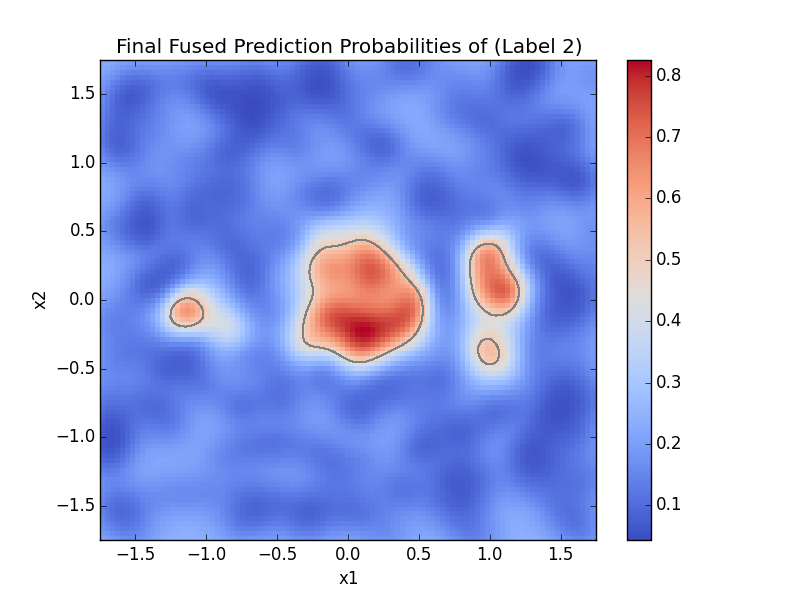
\includegraphics[width = \linewidth]{Figures/scott_reef_modeling/Figure7.eps}
			\caption{Scott Reef: Synthetic Ground Truth}
			\label{Figure:ScottReefSyntheticGroundTruth}
			\end{figure}
			
			\begin{figure}[bp]
			\centering
				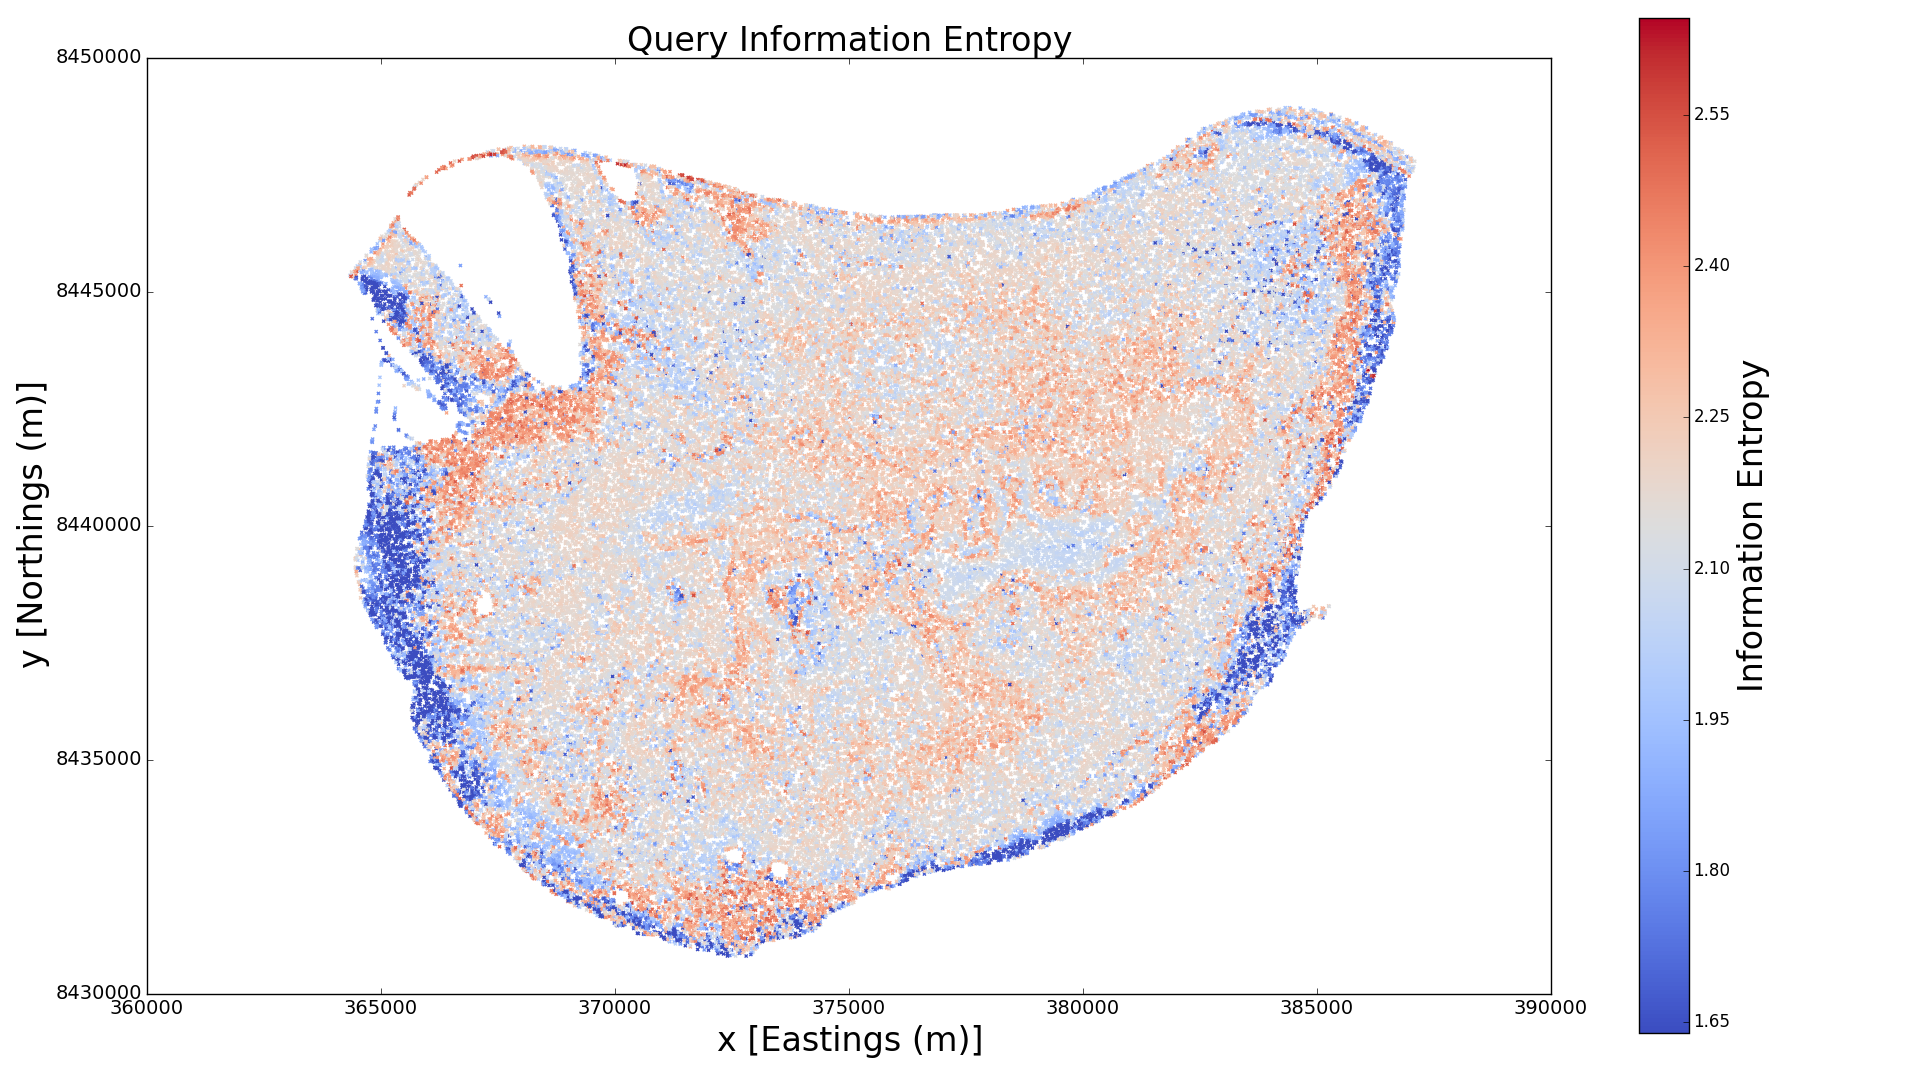
\includegraphics[width = \linewidth]{Figures/scott_reef_modeling/Figure9.eps}
			\caption{Scott Reef: Prediction Information Entropy}
			\label{Figure:ScottReefPredictionInformationEntropy}
			\end{figure}
					
			To reduce computational requirements, 200 training points were sampled from those tracks for initial modeling, which achieves a 41.54\% misclassification rate, or 58.46\% prediction accuracy (figure \ref{Figure:ScottReefInitialPredictions}). This demonstrates the advantage of modeling the benthic environment upon a bathymetric feature space instead of spatial coordinates. The tracks cover less than 5\% of the region, yet more than half of the region can be accurately modeled with such scarce data. This model takes advantage of the fact that although habitats can be far away spatially, they can have similar bathymetric structures such that they are close in the bathymetric feature space.
	
			While we can map the reef with an accuracy of 58.46\% using only 200 training points (figure \ref{Figure:Results:ScottReefInitialPredictions}), the prediction information entropy is rather uniformly high (figure \ref{Figure:ScottReefPredictionInformationEntropy}) due to the scarcity of data. In this initial scenario, under the prediction information entropy criterion the vehicle would simply try to map out all regions as much as possible - a very costly policy.
			
			\begin{figure}[t]
			\centering
				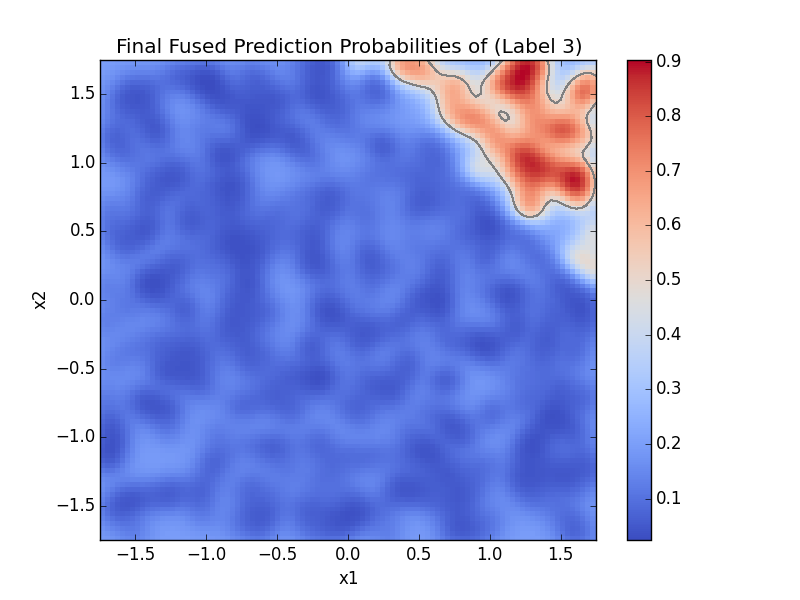
\includegraphics[width = \linewidth]{Figures/scott_reef_modeling/Figure8.eps}
			\caption{Scott Reef: Initial Prediction}
			\label{Figure:ScottReefInitialPredictions}
			\end{figure}
						
			The linearised differential entropy, however, emphasizes on the places where the vehicle should first focus on (figure \ref{Figure:ScottReefLinearisedDifferentialEntropy}). Comparing this with the bathymetric features (figure \ref{Figure:ScottReefBathymetricFeatures}), we can deduce that the vehicle would focus on places with the highest and lowest depths.
			
			\begin{figure}[bp]
			\centering
				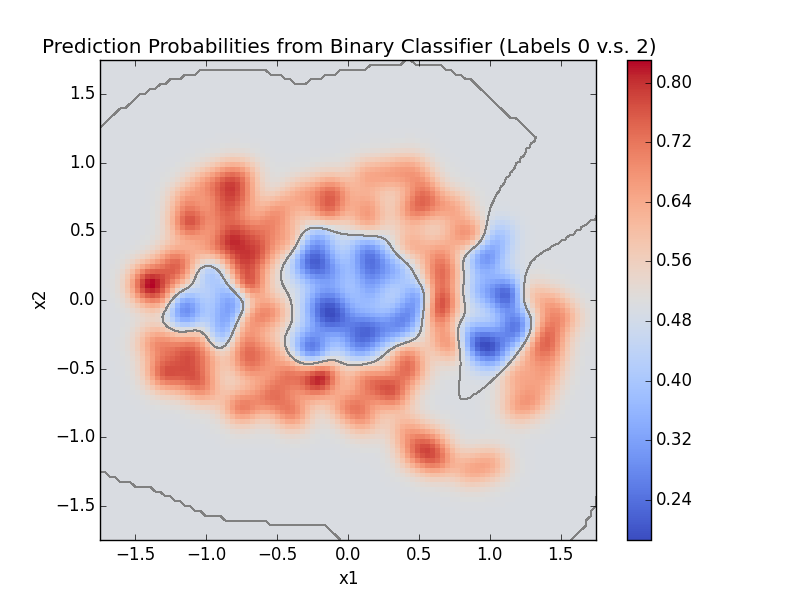
\includegraphics[width = \linewidth]{Figures/scott_reef_modeling/Figure11.eps}
			\caption{Scott Reef: Linearised Differential Entropy}
			\label{Figure:ScottReefLinearisedDifferentialEntropy}
			\end{figure}
			
		\subsection{Problems and Solutions to Big Data Analysis}
		
		\subsection{Feature Extraction}
		
		\subsection{Case with 4 Labels}
		
			(With different amounts of sampled points)
			
		\subsection{Case with 17 Labels}
		